\chapter{Results}\label{chap:results}
We discussed various scenarios in the previous chapter.
In this chapter, we use them to gauge the quality of our numerical scheme.
We start with a convergence test, followed by two standard testing scenarios.
Next, we simulate two different cloud scenarios and check, whether our \amr{} criterion is useful.

\newcommand{\error}{\operatorname{Total-Error}}
\section{Convergence Test}\label{sec:results-convergence}
For the convergence test, we run our manufactured solution scenario~(\cref{sec:manufactured-solution}) for all orders 1 to 6 and for number of cells $3^2, 9^2, 27^2$ and $81^2 $.

Before computing the error we first need to define the $L_p$ norms for a $p > 0$ by
% notation: https://en.wikipedia.org/wiki/Lp_space#Lp_spaces
\begin{equation}
  \label{eq:Lp-nrom}
  \Vert f(x) \Vert_p = \left( \int_K \vert f(x) \vert^p d\mu  \right)^{1/p}.
\end{equation}
We are interested in the total error which we define as the norm of the difference between an analytical solution $f(\bm{x}, t)$ and our approximation $\hat{f}(\bm{x}, t)$.
The error at a time $t$ is thus defined as
\begin{equation}
  \label{eq:error}
  \error(t,p) = \Vert f(\bm{x}, t) - \hat{f}(\bm{x}, t) \Vert_p.
\end{equation}

We first observe that for our approximation space $\broken$ we can split up the error as a sum over all cells.
% \begin{equation}
%   \label{eq:lp-norm-broken}
%  %\Vert f(\bm{x}) \Vert = \sum_{\cell[] \in \broken} \Vert f_{\cell[]} (\bm{x}) \Vert_p,
%   \error(t,p) = \sum_{\cell[] \in \broken} \error_{\cell[]}(t,p)
% \end{equation}
% where $\error_{\cell[]}$ is the error in the cell $\cell[]$.
\todo{Describe how to integrate the error for cells, and effect of volume}
We evaluate the cell-wise error with Gaussian quadrature using \cref{eq:integration-by-substitution}
 \begin{equation}
%   \Vert f(\bm{x}, t) - \hat{f}(\bm{x}, t) \Vert_p^p =
   \error(t,p) = 
   \left( \sum_{\cell[i] \in \broken}
    \left( V \sum_{\bm{j}} \vert f^{\cell[i]}(\bm{x}_j, t) - \hat{f}^{\cell{i}}(\bm{x}_j, t) \vert^p w_{{\bm{j}}} \right) \right)^{1/p}.
 \end{equation}
Here, a superscript of $\cell[j]$ denotes the restriction of the function to a grid cell.
\todo{Use quad node macro here!}
To increase the quality of the error computation, we evaluate both analytical and approximate solution at the quadrature nodes of a scheme with 10 quadrature nodes $x_j$ with weights $w_j$.
We then use these nodes to compute the approximation error per cell.

For the limiting case of $p \to \infty$ we use the maximum point-wise error over all nodal points.

\begin{figure}[htb]
  \centering
  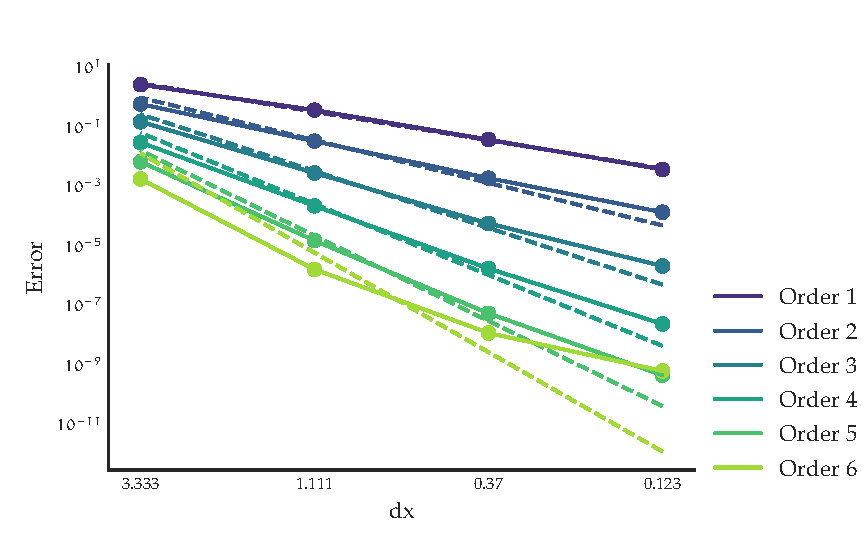
\includegraphics[trim=0.2cm 0.3cm 0.2cm 1.0cm, clip]{thesis_convergence}
  \caption{$L_2$-Error vs.\ Grid Size.
    The dashed lines are the optimal order of convergence $N+1$.
  The line is estimated by using the constant part of a linear regression fit and the ideal order as slope.}
  \label{fig:convergence-l2-error}
\end{figure}

\begin{table}[htb]
  \centering
\caption{Numerical order of convergence of ADER-DG method}%
\label{tab:convergence-order}
\begin{tabular}{@{}lS[table-format=1.2]S[table-format=1.2]S[table-format=1.2]@{}}
\toprule
{Polynomial Order $N$} & {$L_1$} & {$L_2$} & {$L_\infty$}\\ \midrule
1 & 2.03 & 2.00 & 1.92\\
2 & 2.56 & 2.55 & 2.55\\
3 & 3.43 & 3.40 & 3.44\\
4 & 4.27 & 4.27 & 4.36\\
5 & 5.00 & 5.02 & 5.08\\
6 & 4.46 & 4.50 & 4.65\\
\bottomrule
\end{tabular}
\end{table}

To compute the numerical order of convergence, we perform a linear regression of the logarithm of the error vs.\ the logarithm of the meshsize.
The size of the slope is then the convergence order.
Looking at the plot for the $L_2$ error~(\cref{fig:convergence-l2-error}) shows that our method converges for all tested polynomial orders.
Note that the error for the finest grid with order 6 is worse than the error for order 5.
For all other meshsizes and orders, a higher order indicates a smaller error.
If we compare our errors with the optimal order of convergence, we notice that while order 1 exhibits the theoretical order of convergence of 2, larger polynomial orders lead to diminishing returns.

The same is true for other error norms (\cref{tab:convergence-order}).
This means, that we in general do not achieve the optimal theoretical order of convergence.
In~\cite{dumbser2010arbitrary}, which use a similar numerical method and the same scenario, but a different grid, \citeauthor{dumbser2010arbitrary} achieves the optimal order for most polynomial orders.
Some \textsc{dg}-methods of odd order only achieve a numerical convergence order of $N+\nicefrac{1}{2}$.


\section{Accurate CFD}
Show:
\begin{itemize}
\item Taylor-Green High Order
  LIC, Plot v/p ana vs.\ real
\item ABC Medium Order
  Plot p ana.\ vs real
\item Lid-Driven Cavity
  Show LIC, maybe plot over x?
\end{itemize}

\sidetitle{Taylor-Green Vortex}
We use an \aderdg{}-scheme of order 5 with a mesh of size $27 \times 27$ cells to simulate the Taylor-Green Vortex.
The simulation ran for \SI{10}{\s}.
Our solution results in the expected streamlines (\cref{fig:taylor-green-streamlines}).
Furthermore, we compare our results with the analytical solution for the incrompressible case.
We achieve a small error~(\cref{fig:taylor-green-result}) for both pressure and velocity.
The small errors are expected and not only stem from numerical inaccuracies but primarily from the fact that we simulate a compressible fluid.
Note that the error is small over the entire domain, and not only close to the boundary, where we impose the analytical solution.
Overall, we notice a very good agreement with both the results of~\cite{dumbser2016high} and the analytical solution.

\begin{figure}[htb]
  \centering
  \includegraphics[width=0.5\textwidth]{thesis_taylor_green_stream}
  \caption{Streamlines for Taylor-Green vortex}
  \label{fig:taylor-green-streamlines}
\end{figure}

\begin{figure}[htb]
  \centering
  \begin{subfigure}[t]{0.5\textwidth}
    \centering
    \includegraphics{thesis_taylor_green_vel}
    \caption{Position vs.\ velocity}
  \end{subfigure}~%
  \begin{subfigure}[t]{0.5\textwidth}
    \centering
    \includegraphics{thesis_taylor_green_pressure}
    \caption{Position vs.\ pressure}
  \end{subfigure}
  \caption{\label{fig:taylor-green-result}%
    Comparison of Taylor-Green simulation with analytical solution.
    The former is represented by the scatter plot, the latter by the gray line.
    Note that we only show every 5th point.}
\end{figure}

\sidetitle{ABC Flow}
We use an \aderdg{}-scheme of order 2 with a mesh consisting of $27 \times 27 \times 27$ cells to simulate the \textsc{abc}-flow.
We run the simulation for \SI{1}{\s}.
Figure xxx shows two slices of the simulation, figure xxx compares our numerical approximation of the pressure to the analytical solution.
Again, our solution agrees with the analytical solution.
\todo{Velocity?}

\sidetitle{Lid-Driven Cavity}
\begin{figure}[htb]
  \centering
  \begin{subfigure}[t]{0.4\textwidth}
    \centering
    \includegraphics[width=1.2\textwidth]{thesis_lid_driven_cavity_stream}
    \caption{\label{fig:lid-driven-cavity-streamlines}%
      Streamlines of the cavity flow.}
  \end{subfigure}~%
  \begin{subfigure}[t]{0.7\textwidth}
    \centering
    \includegraphics{thesis_lid_driven_cavity}
    \caption{\label{fig:lid-driven-cavity-result}%
      Plot of velocity slices. Lines are our soulution, scatter plot shows reference solution~\cite{ghia1982high}.}
  \end{subfigure}
  
  \caption{Lid-Driven Cavity solution at $t=\SI{30}{\s}$}
  \label{fig:lid-driven-cavity}
\end{figure}

We use a \muscl{}-limited \aderdg{}-scheme of order 3 with a mesh of size $27 \times 27$ for the Lid-Driven Cavity.
The streamlines~(\cref{fig:lid-driven-cavity-streamlines}) agree with the expected solution but have two additional, smaller vortices in the bottom corners.
They do not appear in~\cite{dumbser2010arbitrary} but do appear in~\cite{ghia1982high}.
Additionally, we show the velocity along both axes in \cref{fig:lid-driven-cavity-result}.
They too agree with the reference solution of~\cite{ghia1982high}.

Surprisingly, the limiter was not activated at all.
We noticed that we need the limiter when decreasing the speed of sound. 

\section{Accurate Clouds}
\begin{itemize}
\item Cosine Bubble
\item Two Bubbles
\end{itemize}
The cosine bubble scenario$\ldots$

\sidetitle{Two Bubbles}
We ran the second scenario with the same \amr{} settings as the first one.
The results in (\cref{fig:results-two-bubbles}) are comparable to the reference solution~\cite{muller2010adaptive} for the first seven minutes\todo{Recreate contour plots with amr version!}.
Note that the final plot at \SI{7}{\min} looks different in our simulation.
A possible source for this is that we use a different equation set than~\cite{muller2010adaptive}.
While we use a general purpose set with small modifications for atmospheric flows, they use a equation set that is fully focussed on this scenario.
Furthermore, we use the full Navier-Stokes viscous fluxes instead of an approximation.

\begin{figure}[p]
  \vspace*{-4.5cm}
  \thisfloatpagestyle{empty}
  \centering
  \begin{subfigure}{1\textwidth}
    \centering
    \includegraphics{thesis_two_bubbles_contour_collage.pdf}
  \end{subfigure}
  % \begin{subfigure}[t]{0.5\textwidth}
  %   \centering
  %   \includegraphics[trim=0.0cm 0.0cm 0.0cm 0.8cm, clip]{thesis_two_bubbles_contour_t0}
  % \end{subfigure}~%
  % \begin{subfigure}[t]{0.5\textwidth}
  %   \centering
  %   \includegraphics[trim=0.0cm 0.0cm 0.0cm 0.8cm, clip]{thesis_two_bubbles_contour_t240}
  % \end{subfigure}
  % \begin{subfigure}[t]{0.5\textwidth}
  %   \centering
  %   \includegraphics[trim=0.0cm 0.0cm 0.0cm 0.8cm, clip]{thesis_two_bubbles_contour_t420}
  % \end{subfigure}~%
  % \begin{subfigure}[t]{0.5\textwidth}
  %   \centering
  %   \includegraphics[trim=0.0cm 0.0cm 0.0cm 0.8cm, clip]{thesis_two_bubbles_contour_t600}
  % \end{subfigure}
  \vspace*{1cm}
  \begin{subfigure}[t]{1\textwidth}
    \centering
    \includegraphics[trim=0.0cm 0.0cm 0.0cm 0.0cm, clip, scale=1.2]{giraldo_results_two_bubbles}
  \end{subfigure}
  \caption{\label{fig:results-two-bubbles}%
    Results for two bubble scenario.
    On the top is our, the bottom plots are taken from~\cite{muller2010adaptive}.
  Contour values for potential temperature pertubation are $-0.05, 0.05, 0.1, \ldots 0.45$.
}
\end{figure}

\section{Time-to-solution: AMR vs Static Mesh}\label{sec:results-tts-amr}
To show the effectiveness of the \amr{}, we compare the time to solution of a simulation using \amr{} and another simulation with a fully refined mesh.
In detail, we compare
\begin{description}
\item[AMR] We use a coarse mesh with just $27 \times 27$ cells.
  Each cell can be refined up to three times.
  That is, the cells have sidelengths of roughly $\left(\SI{37.04}{\m}, \SI{12.35}{\m} \right)$.
  As refinement thresholds we use $T_\text{refine} = 2.5$ and $T_\text{delete} = -0.5$ in \cref{eq:refinement-criterion}.
\item[Fine] We use a uniform grid where all cells have a sidelength corresponding to the finest mesh of the \amr{}-test case.
  In addition, we disable the reduction of global observables.
\end{description}
Note, that while our \amr{} criterion is able to cope with an additional, coarser level, the current implementation in \exahype{} is unstable for this scenario.
This is why we only report an \amr{} run with one level of dynamic refinement.

For both settings, we use an \aderdg{}-method of order $4$ and thus have a minimal effective resolution of ca.\ $\SI{3.09}{\m}$.

We use a single node of the Haswell-nodes of the Supermuc (Phase 2).
The node has two Intel® Haswell Xeon Processor E5-2697 v3 \textsc{cpu}s with 14 cores each.
Both \textsc{cpu}s currently run on $\SI{1.8}{\GHz}$.
We use the \tbb{} parallelisation of \exahype{}.
To find a reasonable parameter for the number of background threads, we ran a grid search.
We ran three \amr{} testcases for a simulation time of $\SI{1}{\min}$.
\todo{Noisy, show results}
The best median performance was achieved by using six background threads.

To ensure a fair comparison, we ran both configurations with the same optimisation options:
\begin{verbatim}
"architecture": "hsw",
"shared_memory": {
    "cores": 28,
    "background_job_consumers": 6,
    "properties_file": "sharedmemory.properties",
    "autotuning_strategy": "dummy"
},
"optimisation": {
    "fuse_algorithmic_steps": true,
    "fuse_algorithmic_steps_factor": 0.99,
    "spawn_predictor_as_background_thread": true,
    "spawn_amr_background_threads": true,
    "spawn_update_as_background_thread": true
}
\end{verbatim}
for the time-to-solution test.
For this we ran the simulation without plotters.
The \amr{}-method took \SI{98654.1}{\s} (\SI{1}{\day} \SI{3}{\hour} \SI{24}{\minute} \SI{14}{\s})
while the fully refined grid took \SI{169071}{\s} (\SI{1}{\day} \SI{22}{\hour} \SI{57}{\minute} \SI{51}{\s}).
In other words, the latter method took over 71\% longer.

\section{Reactive Euler \textit{\&} Navier Stokes}
As a final benchmark, we use the reactive Navier-Stokes equations.
We use a limiting \aderdg{}-scheme with an order of 3 and a meshsize of $81 \times 81$.
For some runs, we use the \textsc{cmp}\todo{Refer to dmp equation (and include it)} with the following settings:
\begin{verbatim}
"limiter": {
    "dmp_observables": 3,
    "dmp_relaxation_parameter": 0.05,
    "dmp_difference_scaling": 1e-3,
    "helper_layers": 1
}
\end{verbatim}
We use $\Qrho, \pressure$ and $\QZZ$ as \textsc{dmp} variables.
The results for runs with and without \textsc{dmp} can be seen in figure XXX.
Note, that oscillations diminish the results but are healed by the \textsc{dmp}-criterion.
This scenario shows the differences between the viscous Navier-Stokes equations and the Euler equations clearly:
The viscous effects smooth out the otherwise sharp curves.

It is difficult to compare these results with our references, because they both use different settings.
In constrast to~\cite{helzel2000modified} we use a non-stiff source term and viscous effects, \cite{hidalgo2011ader} includes viscosity but is limited to one-dimensional scenarios.
We can see that our simulation captures the overall behaviour of the reaction similar to~\cite{helzel2000modified} while the viscous effects show the same tendency as the results from~\cite{hidalgo2011ader}.

Plots-TODO:
\begin{itemize}
\item 2D: Mass fraction
\item 2D: Pressure + Limiter
\item 1D: Line plot pressure
\item 1D: Line plot mass fraction
\end{itemize}

\begin{figure}[htb]
  \centering
  \begin{subfigure}[t]{0.3\textwidth}
    \centering
    \includegraphics{thesis_detonation_euler_nodmp_pressure}
    \caption{Pressure, Euler, no \textsc{dmp}}
  \end{subfigure}~%
  \begin{subfigure}[t]{0.3\textwidth}
    \centering
    \includegraphics{thesis_detonation_euler_dmp_pressure}
    \caption{Pressure, Euler, \textsc{dmp}}
  \end{subfigure}~%
  \begin{subfigure}[t]{0.3\textwidth}
    \centering
    \includegraphics{thesis_detonation_ns_pressure}
    \caption{Pressure, \textsc{NS}, no \textsc{dmp}}
  \end{subfigure}

  \begin{subfigure}[t]{0.3\textwidth}
    \centering
    \includegraphics{thesis_detonation_euler_nodmp_Z}
    \caption{$Z$, Euler, no \textsc{dmp}}
  \end{subfigure}~%
  \begin{subfigure}[t]{0.3\textwidth}
    \centering
    \includegraphics{thesis_detonation_euler_dmp_Z}
    \caption{$Z$, Euler, \textsc{dmp}}
  \end{subfigure}~%
  \begin{subfigure}[t]{0.3\textwidth}
    \centering
    \includegraphics{thesis_detonation_ns_Z}
    \caption{$Z$, \textsc{NS}, no \textsc{dmp}}
  \end{subfigure}
  
  \caption{\label{fig:detonation-line-plots}%
    Slices along the $x$-axis for our three configurations.
    We only show one half of the slice because the scenario is symmetric.
  }
\end{figure}

%%% Local Variables:
%%% mode: latex
%%% TeX-master: "../main"
%%% End:
